\chapter{Experimental Models}
\label{Chap:3}
\hspace{0.5cm} In this chapter, we are going to study the architectures and the algorithms of DeepSORT\cite{Wojke2017simple}
and propose two architecture alterations to the DeepSORT\cite{Wojke2017simple} with expectations to improve the performance of original method.

\section{DeepSORT}
\subsection{Workflows}
\hspace{0.5cm} DeepSORT\cite{Wojke2017simple} is a tracking-by-detection framework for the problem of multiple 
object tracking (MOT) where objects are detected in each frame and presented as bounding boxes \cite{sort}.\par
\begin{figure}[h!]
    \centering
    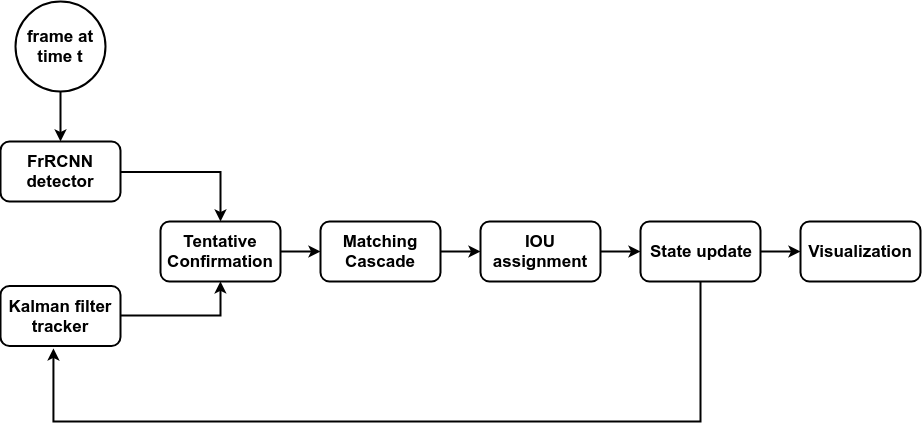
\includegraphics[width=\textwidth]{Chapters/Fig/Thesis_diagram-DeepSORT.png}
    \caption{DeepSORT workflow diagram}
    \label{fig:deepsort_workflow}
\end{figure}
In DeepSORT, for the tracking part, \cite{Wojke2017simple} uses Faster \acrshort{RCNN} detector which has been pretrained on a collection of public and private datasets to provide excellent performance \cite{Wojke2017simple}, while in the tracking part, \cite{Wojke2017simple} uses a standard Kalman filter with constant velocity motion and linear observation model. The bounding coordinates $(u,v,\gamma,h)$ are taken as direct observations of the object state where $u,v$ is the bounding box center, $\gamma$ is the aspect ratio and $h$ is the height.\par
The results of tracking and detecting go through a tentative confirmation, then forward to two matching gates; 
firstly, \textit{Matching cascade}, workflow diagram of which shown in fig.\ref{fig:org_matching_cascade},
 secondly, \textit{\acrshort{IoU} assignment} workflow diagram of which shown in fig.\ref{fig:org_iou}\par.
\begin{figure}[h!]
    \centering
    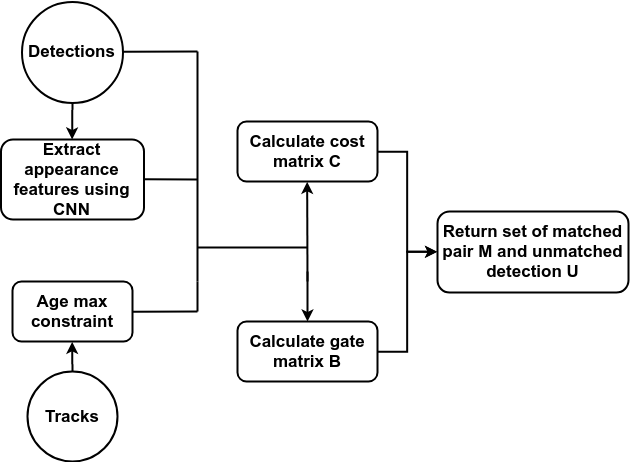
\includegraphics[width=0.8\textwidth]{Chapters/Fig/Thesis_diagram-CNN_Matching_Cascade.png}
    \caption{DeepSORT matching cascade}
    \label{fig:org_matching_cascade}
\end{figure}
\begin{figure}[h!]
    \centering
    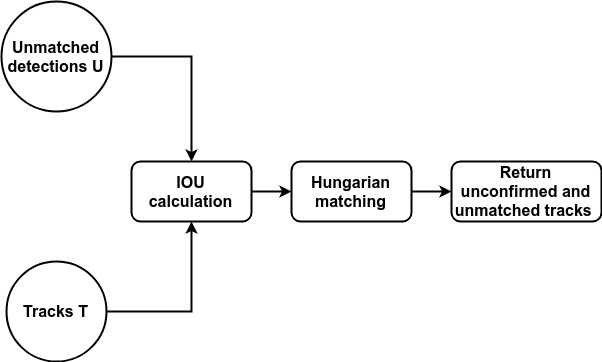
\includegraphics[width=0.8\textwidth]{Chapters/Fig/Thesis_diagram-IOU.png}
    \caption{DeepSORT \acrshort{IoU} assignment}
    \label{fig:org_iou}
\end{figure}

\pagebreak
\cite{Wojke2017simple} defines some constraints to match and suppresses the detections and tracks:
\begin{itemize}
    \item For each track $k$, a number $a_k$ is the number of frames since the last successful measurement. This counter is incremented during Kalman filter prediction and assign to be zero when the track is associated with a measurement.
    \item Tracks that exceed a predefined maximum age $A_{max}$ are considered being deleted from the track set.
    \item New track hypotheses are initiated for each detection that cannot be associated to an existing track.
    \item New tracks are classified as tentative during their first three frames, during first three frames, a successful measurement association at each time step, if not, the track will be deleted.
\end{itemize}
\subsection{Motion information measurement}
\hspace{0.5cm} \cite{Wojke2017simple} proposed to use the Mahalanobis distance between predicted Kalman states and the newly arrived measurement
\begin{equation}
    d^{(1)}(i,j) = (d_j - y_i)^TS^-1_i(d_j-y_i)
\end{equation}
where $d_j$ indicates the position of the $j$-th detection box, $y_i$ indicates the predicted position of the $i$-th 
tracker to the target, $S_i$ indicates the co-variance matrix between the detected position and the average tracking position. \
The Mahalanobis distance takes into account the uncertainty of the state measurement by calculating the standard deviation between the detected position and the average tracking position.\par
If the Mahalanobis distance is less than a specified threshold $t^{(1)}$, the association is denoted by this binary indicator:
\begin{equation}
    b^{(1)}_{i,j}=\mathbb{1}[d^{(1)}(i,j) \leq t^{(1)}]
\end{equation}
$t^{(1)}$ is default set to 9.4877.\cite{Wojke2017simple}
\subsection{Appearance information measurement}
\hspace{0.5cm} Since the Mahalanobis distance provides only a rough estimate of object location, when motion uncertainty is high or occlusions occurs, motion information measurement is not enough. Hence, \cite{Wojke2017simple} proposed a second measurement using appearance features.\par
\begin{itemize}
    \item For each bounding box detection in $d_j$ an appearance descriptor $r_j$ that is calculated from a  \acrshort{CNN} model, 
    the architecture of which is shown on tab.\ref{tab:cnn_deepsort_arch}, pre-trained on a large-scale re-identification dataset Market1501
    
    \item For a track $k$, keep a gallery $\mathcal{R}_k$ that stores feature vector of detection results for the last 100 frames that each tracking target successfully associated with.
     Then calculate the cosine distance between the $i$-th track and $j$-th detection in the appearance space:
    \begin{equation}
        d^{(2)}(i,j) = min\{1 - r_j^Tr^{(i)}_k | r^{(i)}_k\in \mathcal{R}_i\}
    \end{equation}
    \item A binary variable to indicate if an association is admissible to this metric:
    \begin{equation}
        b^{(2)}_{i,j}=\mathbb{1}[d^{(2)}(i,j) \leq t^{(2)}]
    \end{equation}
    $t^{(2)}$ is obtained from a separate training set
\end{itemize}
\hspace{0.5cm}The Mahalanobis distance provides information about possible object locations based on motion that are particularly useful for short-term predictions. On the other hand, the cosine distance considers appearance information that are particularly useful for recover ids after long-term occlusion.\par
Two metrics are combined by a weighted sum:
\begin{equation}
    c_{i,j} = \lambda d^{(1)}(i,j) + (1-\lambda)d^{(2)}(i,j)
\end{equation}

The association is admissible if it is within the gate regions of both metrics:
\begin{equation}
    b_{i,j}=\Pi^2_{m=1}b^{(m)}_{i,j}
\end{equation}\par
In practical, the hyperparameter $\lambda$ is set to 0. Only appearance information are used in the association cost term when the Mahalanobis is useful in disregarding infeasible assignments inferred by the Kalman filter.
\begin{table}[H]
\begin{center}
 \begin{tabular}{||c c c ||} 
 \hline
 Name & Patch size/Stride & Output size \\ [0.5ex] 
 \hline\hline
 Conv1 & 3x3/1 & 32x128x64  \\ 
 Conv2 & 3x3/1 & 32x128x64 \\
 Max Pool 3 & 3x3/2 & 32x64x32 \\
 Residual 4 & 3x3/1 & 32x64x32 \\
 Residual 5 & 3x3/1 & 32x64x32 \\
 Residual 6 & 3x3/1 & 64x32x16 \\
 Residual 7 & 3x3/1 & 64x32x16 \\
 Residual 8 & 3x3/1 & 128x16x8 \\
 Residual 9 & 3x3/1 & 128x16x8 \\
 Dense 10   &       & 128    \\
 Batch and $\mathnormal{l}_2$ normalization &  & 128 \\
 \hline

 \hline
\end{tabular}
\end{center}
    \caption{CNN architecture of deep feature extractor in DeepSORT}
    \label{tab:cnn_deepsort_arch}
\end{table}\pagebreak
\subsection{Matching Cascade}
\begin{algorithm}
\caption{Matching Cascade}\label{algo:ds_matching}
\begin{algorithmic}[1]
\INPUT Tracking indices $\mathcal{T} = \{1, .. N\}$, Detection indices $\mathcal{D} = \{1, .. M\}$, Maximum age $A_{max}$

\State Compute cost matrix $\mathbf{C} = [c_{i,j}]$ using in Eq 3.3
\State Compute gate matrix $\mathbf{B} = [b_{i,j}]$ using in Eq 3.4
\State Initialize set of matches $\mathcal{M} \leftarrow \emptyset$
\State Initialize set of unmatched detection $\mathcal{U}\leftarrow\mathcal{D}$
\For{$n \in \{1, .., A_{max}\}$}
\State Select tracks by age $\mathcal{T}_n \leftarrow \{i \in \mathcal{T} | a_i = n\}$
\State $[x_{i,j}]\leftarrow$ min\_cost\_matching($\mathbf{C}, \mathcal{T}_n, \mathcal{U})$
\State $\mathcal{M} \leftarrow \mathcal{M} \cup \{(i,j) | b_{i,j}\cdot x_{i,j} > 0 \}$
\State $\mathcal{U} \leftarrow \mathcal{U}$ /\ $\{j |\underset{i}{\sum}b_{i,j}\cdot x_{i,j} > 0 \}$
\EndFor
\State Return $\mathcal{M}, \mathcal{U}$
\end{algorithmic}
\end{algorithm}
When an object is occluded for a longer period of time and two tracks compete for the same
detection, the Mahalanobis distance favors uncertainty, because it effectively reduces the
distance in the standard deviation of any detection toward the projected
track mean which can lead to increase track fragmentation and unstable tracks.\cite{Wojke2017simple}
Wojke et al.\cite{Wojke2017simple} introduced a matching cascade shown in algo.\ref{algo:ds_matching}
that gives priority to more frequently seen objects.\par
The subset of tracks $\mathcal{T}_n$ that have not been associated in last $n$
frames is considered to estimate linear assignment between tracks in $\mathcal{T}_n$ and undetected
detection $\mathcal{U}$. The matching cascade algorithm return set of matches and unmatched
detection. Then, to the final stage, using \acrshort{IoU} with Hungarian
algorithms to associate unmatched and unconfirmed track at age $n=1$ and the unmatched detection. This helps to to account for sudden appearance changes, e.g., due to partial occlusion with static scene geometry, and to
increase robustness against erroneous initialization\cite{Wojke2017simple}.\par



\section{DeepSORT with Parameter-free Spatial Attention to extract deep appearance features}
\hspace{0.5cm} One of the most difficult problem to handle in pedestrian tracking is re-identification. Re-identification problem comes from the limitation of
\acrshort{FOV} of camera, partially or fully occlusion and
reappearance . In the DeepSORT \cite{Wojke2017simple}, authors proposed an
appearance metric that uses feature vectors extracted from a \acrshort{CNN} to compare to
gallery of features of successfully tracked objects from 100 previous
frames in order to identify current target. However, the \acrshort{CNN} architecture is simple and do not archive competitive result on these
re-identification datasets, theoretically, replacing mentioned \acrshort{CNN}
architecture by a stronger or better model in person re-identification
challenge would provide a more accurate measurement to re-identify pedestrian.\par

\begin{figure}[h!]
    \centering
    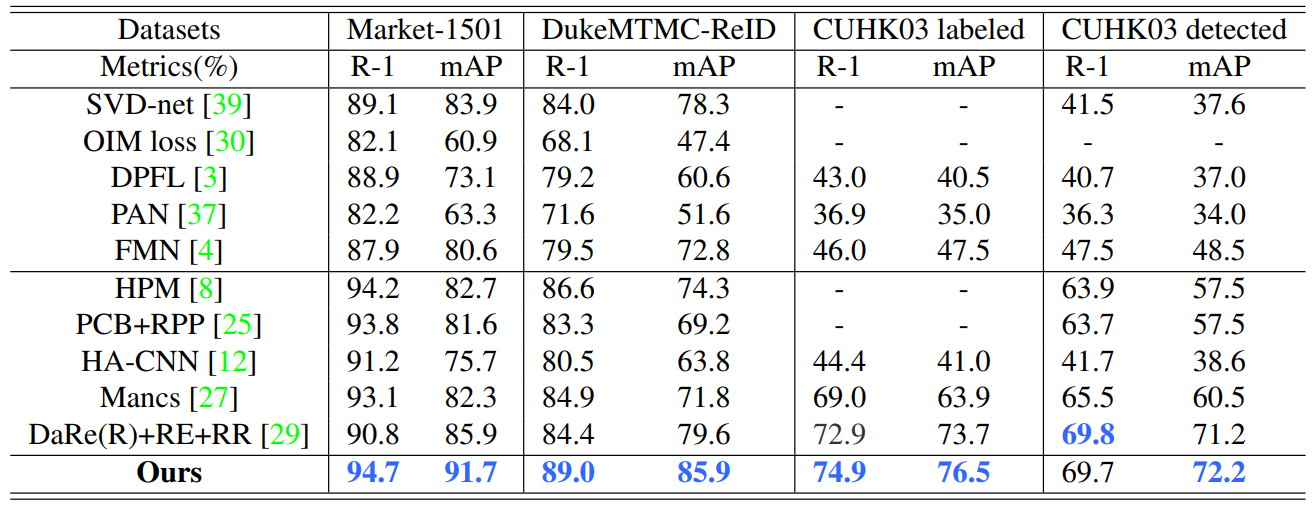
\includegraphics[width=0.8\textwidth]{Chapters/Fig/person-re-id-performance.png}
    \caption{Results of Parameter-free Spatial Attention Network for Person Re-identification in large-scale person re-identification dataset,
    \textbf{Ours} denoted for \cite{SA}}
    \label{fig:sa_results}
\end{figure}
The \cite{SA} currently provides state-of-the-art results which is shown in fig.\ref{fig:sa_results} on almost large-scale person
re-identification dataset.Combining the idea of using a better architecture in person re-identification problem to extract feature vector and the state-of-the-art performance of
\cite{SA} in person re-identification problem, we would like to propose an architecture with the baseline based on \cite{Wojke2017simple} integrating with \cite{SA}
in the \textit{Appearance information measurement} state or DeepSORT with Parameter-free Spatial Attention for extracting appearance features (SADeepSORT). The workflow diagram of SADeepSORT is shown
in fig.\ref{fig:sa_matching}. 
% Comparitive results of SADeepSORT and DeepSORT \cite{Wojke2017simple} in the \autoref{Chap:4}. 
\begin{figure}[h!]
    \centering
    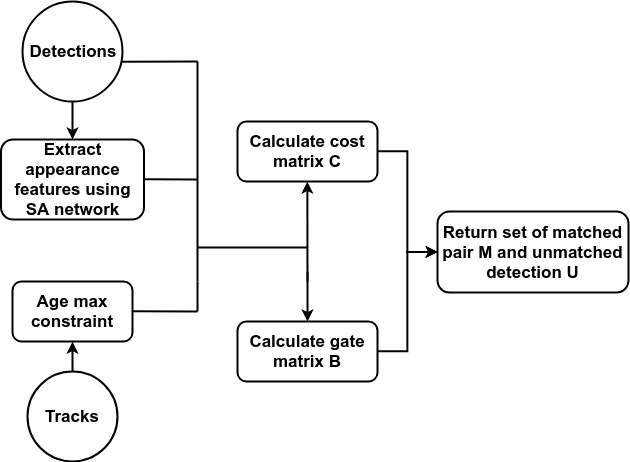
\includegraphics[width=0.8\textwidth]{Chapters/Fig/Thesis_diagram-SA_Matching_Cascade.png}
    \caption{Spatial Network in Matching Cascade of DeepSORT framework}
    \label{fig:sa_matching}
\end{figure}

\pagebreak
\section{DeepSORT with YOLOv3 detector}

\begin{figure}[h!]
    \centering
    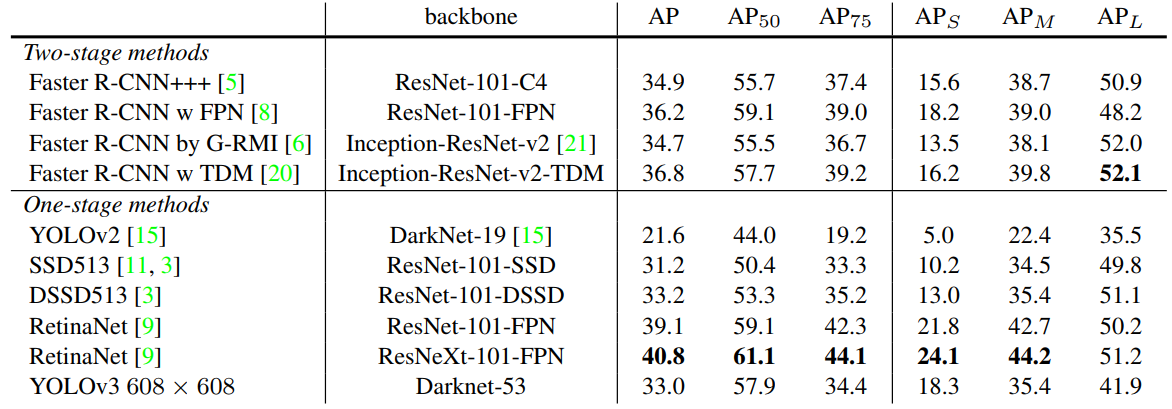
\includegraphics[width=0.8\textwidth]{Chapters/Fig/yolov3_acc_com.png}
    \caption{Accuracy of objects detection algorithms on COCO dataset}
    \label{fig:yolov3_acc_com}
\end{figure}
Fig.\ref{fig:yolov3_acc_com} \cite{yolov3} is showing the result of detection algorithms on COCO dataset,
\cite{yolov3} argues that YOLOv3 is much better than SSD variants and comparable to state-of-the-art
models on the $\text{AP}_{50}$ metric while the computational time is much faster.\par
For the online tracking problem, time constraint is very important, moreover, the quality of the detector makes a proportional effect to the performance of the tracking framework.\par
For all the reasons, we would like to propose DeepSORT with YOLOv3 detector (YOLOv3-DeepSORT), the baseline of YOLOv3-DeepSORT now is shown in the fig.\ref{fig:yolo_deepsort} 
\begin{figure}[h!]
    \centering
    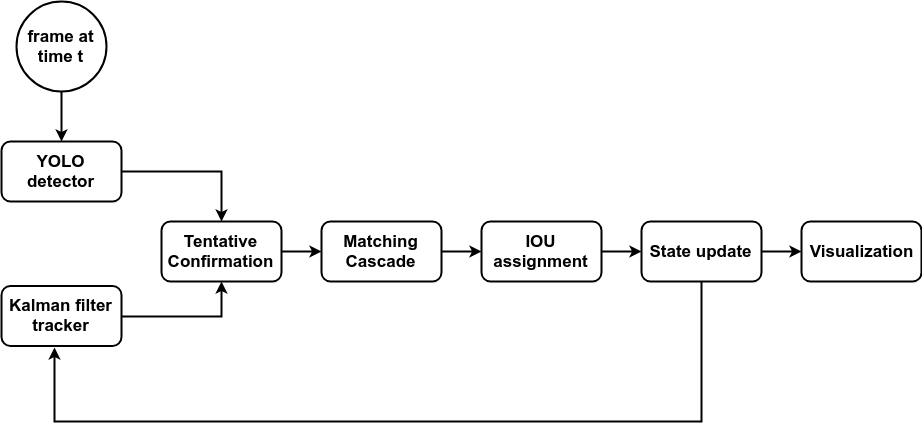
\includegraphics[width=0.8\textwidth]{Chapters/Fig/Thesis_diagram-yolo_deepsort.png}
    \caption{YOLO-DeepSORT's workflow}
    \label{fig:yolo_deepsort}
\end{figure}
